\documentclass[12pt, oneside]{article}
\usepackage[letterpaper, margin=1in, headsep=0.5in]{geometry}
\usepackage[english]{babel}
\usepackage[utf8]{inputenc}
\usepackage{amsmath}
\usepackage{amsfonts}
\usepackage{amssymb}
\usepackage{tikz}
\usepackage{tkz-fct} %alternative to pgfplots.
\usepackage{pgfplots}
\pgfplotsset{width=10cm,compat=1.9}
\usepgfplotslibrary{statistics}
\usepackage{pgfplotstable}
%\usepackage{venndiagram}

\usepackage{fancyhdr}
\pagestyle{fancy}
\fancyhf{}
\rhead{\thepage \\Name: \hspace{1.5in}.\\}
\lhead{BECA / Dr. Huson / 12.1 IB Math\\* Template geometric figures}

\renewcommand{\headrulewidth}{0pt}

\begin{document}
\subsection*{Graphs}
Directions
\begin{flushright} 1.1 \end{flushright}

%Graph / grid
\begin{center}
    
\begin{tikzpicture}
    \draw[step=0.25in,gray,very thin] (0,0) grid (12.7,12.7);
    \end{tikzpicture}
\end{center} %Regents style, no axes
\newpage

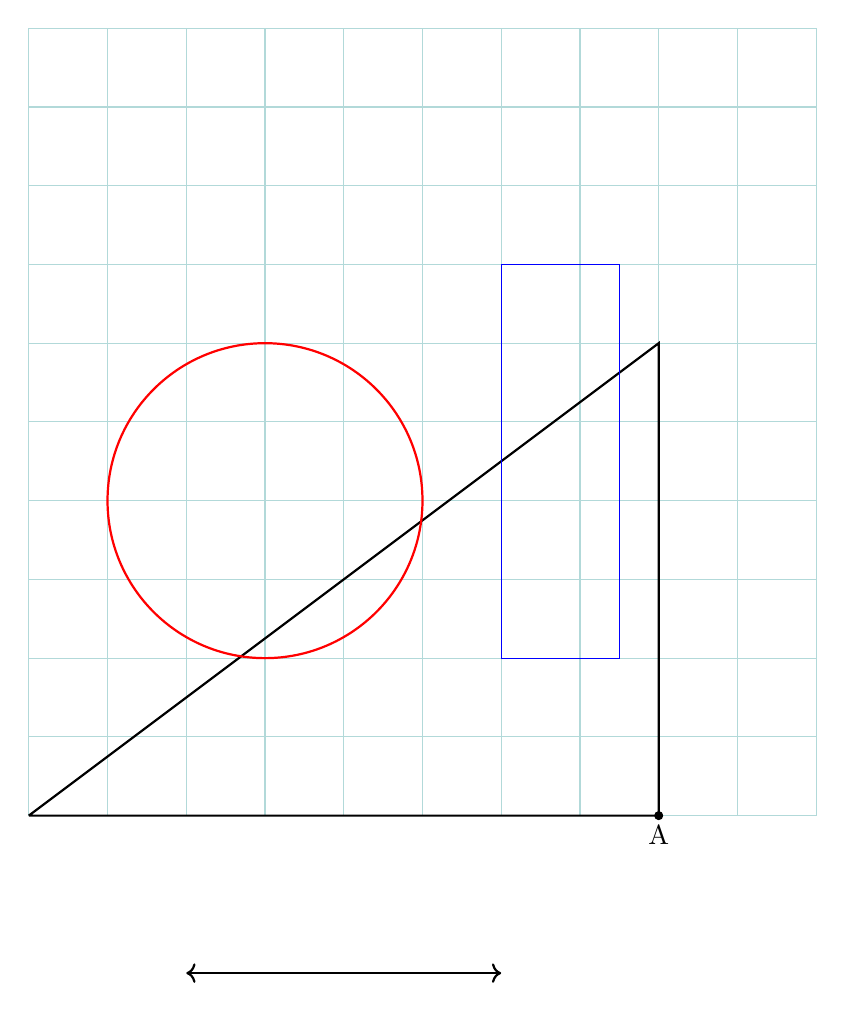
\begin{tikzpicture}[xscale=1,yscale=1] % or scale=3 for both
  \draw[help lines] (0,0) grid (10,10);
  \draw [thick](0,0)--(8,0)--(8,6)--(0,0);
  \draw [fill] (8,0) circle [radius=0.05];
  \node [below] at (8,0) {A}; %above, right, left
  \draw [<->, thick] (2,-2)--(6,-2); % also thin, ultra thick, help lines, dashed, dotted, red
  \draw [blue] (6,2) rectangle (7.5,7);
  \draw [red, thick] (3,4) circle [radius=2];
\end{tikzpicture}

\begin{tikzpicture}
  \draw [thick, <->] (0,5) node [left] {$y$}
       -- (0,0) -- (5,0) node [below right] {$x$};
  \draw[fill] (2,2) circle  [radius=0.05]
       node[below left] (2, 2) {$A$};
  \draw [thick] (2,2)--(5,2) node[right] {$C$} --(5,4) node[right] {$B$} --(2,2);
  \draw [thick] (3.5,2.1)--(3.5,1.9);
  \node [right] at (5,3) {$BC=2$};
\end{tikzpicture}


\begin{center}
\begin{tikzpicture} %pgfplots
\begin{axis}[axis lines = none]
  \addplot[ mark=* ] coordinates {(0,0)(8,0)(8,6)};
\end{axis}
\end{tikzpicture}
\end{center}

\newpage

\begin{tikzpicture}
\begin{axis}[
    title = {Title: pgfplots coordinates plot},
    axis lines = center, %left, %box, left, middle, center, right, none
    xlabel = $x$,
    ylabel = {$y$},
    xmin=-10, xmax=10,
    ymin=-10, ymax=10,
    %xtick={0,2,4,6,8,10},
    %xmajorgrids=true,
    %grid style=dashed
]
\addplot[ mark=* ] coordinates {(1,2)(-3,5)(4,4)};
    %brackets are mandatory, leave blank space
\end{axis}
\end{tikzpicture}


\end{document}
